%!TEX root = ../Thesis.tex
\chapter{Performance Assessment \& Verification of Aggregator Services} % (fold)
\label{cha:verification}
\begin{marginfigure}
	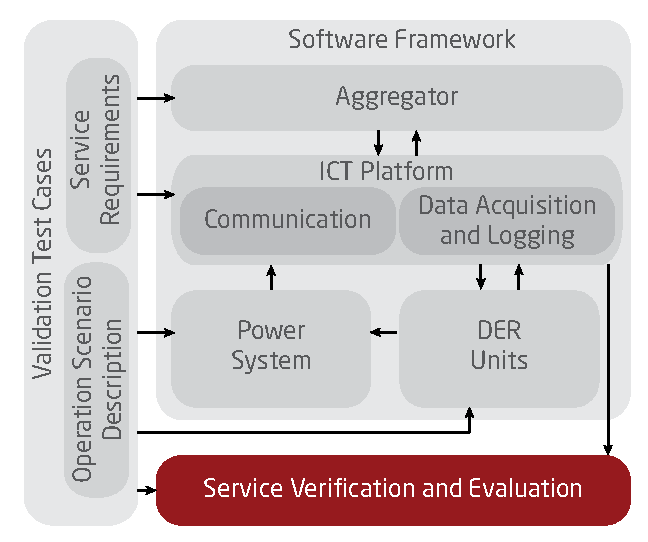
\includegraphics[width=\textwidth]{framework_verification.eps}
	\caption{This chapter focuses on the \emph{service verification and evaluation} block of the aggregator validation framework presented in Chapter~\ref{cha:validation}.}
      \label{fig:frameworkverification}
\end{marginfigure}
\newchapter{P}{erformance assessment is the} process\marginnote{The IEEE defines verification as:``confirmation, through the provision of objective evidence, that specified requirements have been fulfilled.''} of quantifying and verifying the provision of a service according to the contractual specifications of the service. Performance assessment usually occurs at three stages\fcite{coalition2014mapping}
\begin{itemize}
	\item To qualify potential resources against service specifications as part of the validation/prequalification procedure.
	\item To verify service conformance to the service specifications during and after service delivery. 
	\item To calculate the amount of service delivered by the resource as part of financial settlements.
\end{itemize}
%\begin{itemize}
%	\item Why is verification an important part of validation?
%	\item Performance Assessment of Aggregators providing Demand Response
%\end{itemize}
%All resources should be held to the performance specifications established by the product. However – demand side and generation side communication requirements will usually need to be designed separately and made appropriate to each. Technical rules often proscribe the use of metered values to base performance and settlements.[from the SEDC report used in the DRAS paper]

This chapter presents a novel set of performance indices developed for aggregator performance assessment which can be applied at the three stages outlined above. The main focus of the results presented is on aggregator validation and service verification. \todo{finish thought here\ldots something about the importance or the relevance}

The initial work on aggregator performance assessment was presented in a conference paper\fcite{bondy2014performance} and further refined in a submitted journal paper\fcite{bondy2016method}. These paper can be found in Appendix~\ref{app:isgt2014} and Appendix~\ref{app:segan}. 


\section{Background}
\newsection{L}{ittle attention has been} given to the problem of performance assessment of aggregator controllers seen from a service-delivery perspective. As stated in Section~\ref{subsec:aggtest}, performance assessment of aggregators has been mostly ad-hoc analysis specific to a problem the designers are trying to solve, but none have taken a systematic approach to the evaluation of aggregators in terms of established service requirements. In this section we present the concept of control performance assessment and performance indices in power systems, which are topics that serve as background for the rest of the chapter.

\subsection{Control Performance Assessment}
Control Performance Assessment (CPA) is already an established field within control engineering. Most of the applications within the field are found in the process industry\fcite{jelali2006overview}, but since aggregators are a control system, and provide control services, it is natural to translate concepts of CPA to the power system. Usually, CPA methods fall within two types:
\begin{itemize}
	\item benchmarking of controllers towards a theoretic optimum, taking stochasticity of the process into account; and
	\item benchmarking against deterministic properties required of the close-loop system.
\end{itemize}

Usually these indices are normed so that for an index $\eta$:
\begin{equation}
	\eta \in [0,1].
\end{equation}

\subsection{Performance Indices in the Power System}
Currently, the concepts of performance indices and evaluation criteria are used in the power system for the general assessment of how well the System Operator is managing the system. But these evaluation concepts are usually tailored to specific services, \eg CPS1 and CPS2\footnote{An alternative to these two Control Performance Standards is formulated in \cite{gross2001analysis}.} used by NERC\fcite{nerc2011balancing} for evaluating regulation, or the \emph{nadir-based frequency response} metric\fcite{eto2010use} used for evaluating the quality of primary frequency control in an area. Other evaluation criteria have the power interruption to the end customer in focus, \eg System Average Interruption Duration Index (SAIDI) and System Average Interruption Frequency Index (SAIFI)\fcite{LaCommare20061845}. 

As part of the FERC order 755\footnote{The order stipulates that all units providing regulation should get remunerated based upon their performance.}, PJM has introduced a performance score for the remuneration of services in the form of:
\begin{equation}
	\text{Performance Score} = A S_A + B S_D +C S_P
\end{equation}
where $S_A$ is an accuracy score, $S_D$ is a delay score, $S_P$ is a precision score, and $A+B+C =1$ are scalar weights. While this is a detailed performance metric, it is tied to the way LFC is done in PJM. \todo{refine thought, and see where LFC is defined for the first time, probably should be in the services section}

A measure for the performance of aggregators, that is not directed at a single service and that has service delivery in focus, is the topic of this chapter.

\section{Quality of Service}\label{sec:MAINQoS}
\newsection{T}{he concept of Quality}\marginnote{This section relies heavily on the service modeling concepts presented in Chapter~\ref{cha:services}, and it is recommended that the reader familiarizes with that section before reading this section.} of Service (QoS) is closely related to the service models presented in Section\bondy{put in correct section reference}. One of the elements of a service model is the definition of the service error. QoS is an instantaneous measure of how well the aggregator is delivering a service at any given time instant, and can be defined as the scaling of the error to the limits defined in the service model, \ie:
\begin{equation}
	QoS(t) = e(t)C_s(t),
\end{equation}
where $e(t)$ is the error in service delivery and $C_s(t)$ is a time varying normalization factor. This factor ensures that:
\begin{itemize}
	\item $QoS \geq 0$,
	\item for $QoS \leq 1$ the service is considered delivered within the contractual constraints, and
	\item $QoS = 0$ is a perfect service delivery.
\end{itemize}

The original definition proposed in \cite{bondy2014performance} assumed symmetric constraints around the acceptable provision, but in \cite{bondy2016method} this definition was expanded to account for asymmetry, thus $C_s(t)$ is defined as:
\begin{equation}
C_{s}(t) = 
\begin{cases}
\frac{1}{x_{acc,max}(t) - x_{max}(t)}, & e(t) \geq 0 \\
\frac{1}{x_{acc,min}(t) - x_{min}(t)}, & e(t) < 0.
\end{cases}\label{eq:MAINcst}
\end{equation}
where $x_{acc,max/min}$ and $x_{max/min}$ are part of the service model defined in Section~\bondy{refer to correct section}. A visual representation of the error models and their corresponding \emph{QoS} definition are shown in Figure~\ref{fig:MAINerrorQoS}

\begin{figure}[htpb!]
\centering
\subfloat[Tracking service error]{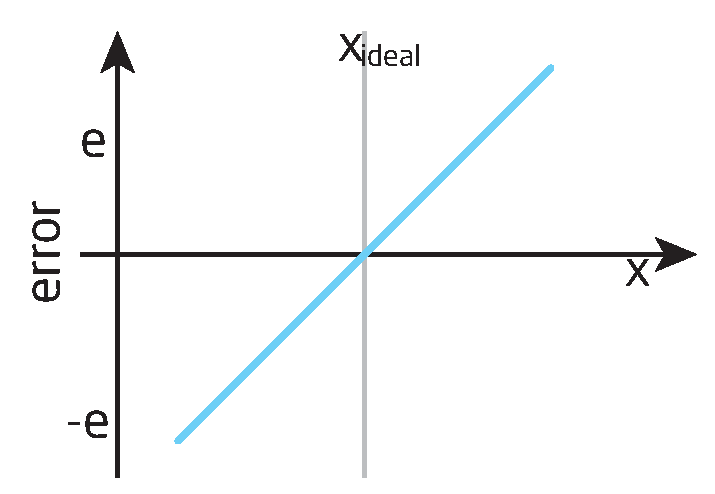
\includegraphics[width=0.5\columnwidth]{SEGAN/tracking_error2.eps}%
\label{subfig:errortracking}} \subfloat[Tracking service Quality of Service]{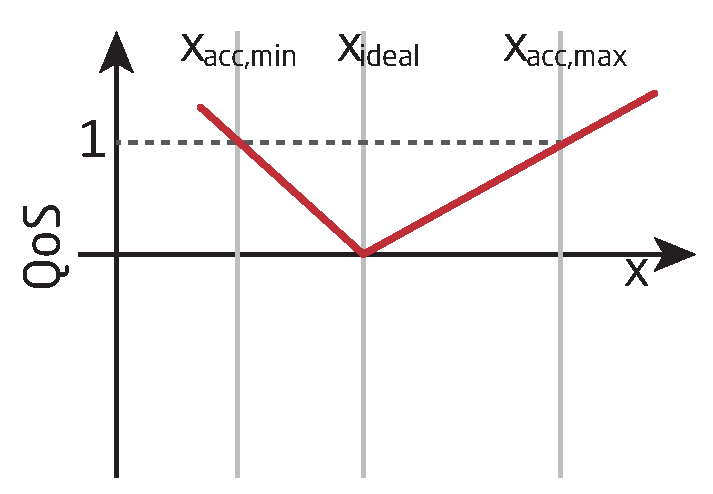
\includegraphics[width=0.5\columnwidth]{SEGAN/tracking_error3.eps}%
\label{subfig:qostracking}}\\
\subfloat[Band service error]{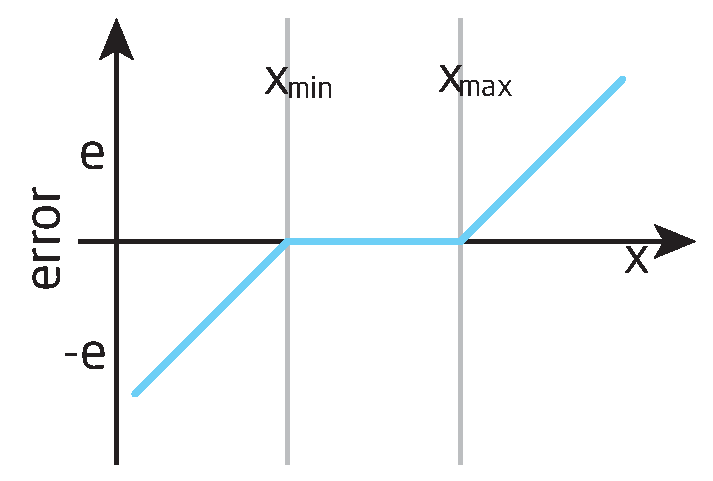
\includegraphics[width=0.5\columnwidth]{SEGAN/band_error2.eps}%
\label{subfig:errorband}}\subfloat[Band service Quality of Service]{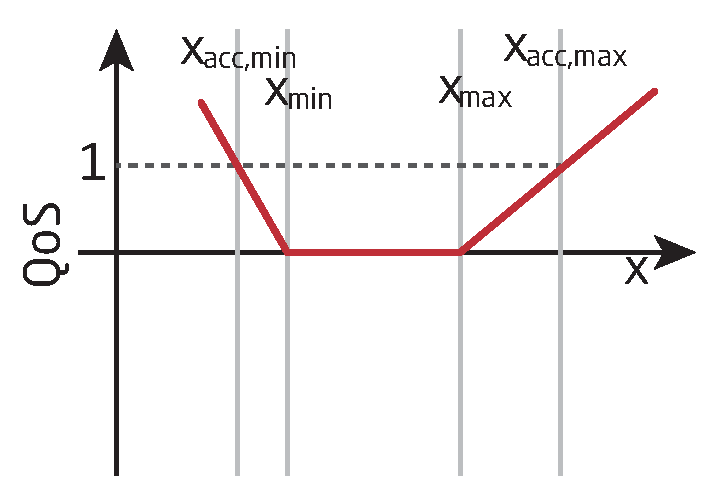
\includegraphics[width=0.5\columnwidth]{SEGAN/band_error3.eps}%
\label{subfig:qosband}}\\
\subfloat[Cap service error]{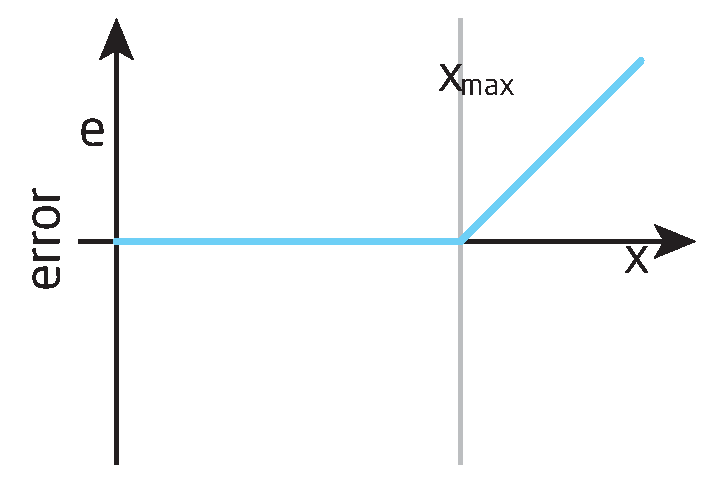
\includegraphics[width=0.5\columnwidth]{SEGAN/cap_error2.eps}%
\label{subfig:errorcap}}
\subfloat[Cap service Quality of Service]{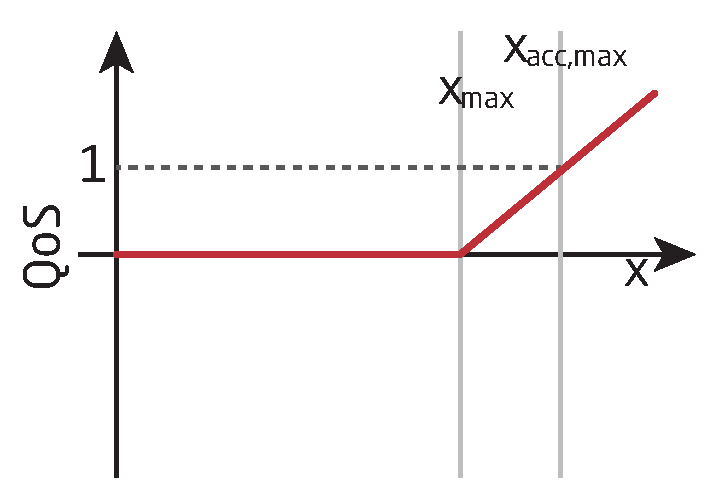
\includegraphics[width=0.5\columnwidth]{SEGAN/cap_error3.eps}%
\label{subfig:qoscap}}
\caption{Error and QoS for the three kinds of services, note that the acceptable band do not need to be symmetric.}
\label{fig:MAINerrorQoS}
\end{figure}

\section{The Aggregator Performance Indices}
\newsection{P}{erformance criteria used for} evaluating controllers usually fall within three categories\fcite{Green}: quality, reliability and energy efficiency. When assessing aggregators, service quality and service reliability define the performance of the aggregator. Four requirements are defined for the performance criteria of aggregators:
\begin{itemize}
	\item[R1] Provide a \emph{quality} measure normalized to the contractual requirements (bounds) of a service. 
	\item[R2] The measure should be normalized with respect to time.
	\item[R3] Provide a \emph{reliability} measure in relation to service non-delivery.
	\item[R4] Each service that the aggregator provides must have a separate, individually verifiable, measure. For example, to evaluate service delivery with respect to ancillary-service delivery, the asset-management quality is irrelevant.
\end{itemize}

To fulfill these requirements two indices are defined:
\begin{itemize}
	\item a service performance assessment index, and
	\item a service verification index.
\end{itemize}

\subsection{Service Performance Assessment index}
The service performance assessment index consists of the weighted average of the normalized root mean square error (RMSE) of the service delivery\footnote{Originally, this index was defined in \cite{bondy2014performance} as the integral square error (ISE) of the service delivery, which was then normalized to a maximum allowable error. This definition does note cope well when the service provision of several services are evaluated at the same time. Therefore, the index was reformulated as the RMSE.}. For evaluation of \emph{K} amount of ancillary services, over discrete time horizon of service delivery \emph{N}, the index is defined:
\begin{align}\label{eq:MAINetaAS}
\eta^{AS} &= \sum^{K}_{i=1} W^{AS}_i \sqrt{\frac{\sum^{N_i}_{t=0} \left( {QoS^{AS}_{i,t}}^{2} \right)}{N_i}}\\
\sum_{i=1}^K W^{AS}_i &= 1 \label{eq:was}
\end{align}
where $QoS^{AS}_{i,t}$ is the truncated $QoS \in [0,1]$ of the ancillary serviced delivery. This definition means that $\eta^{AS} \in [0,1]$, where values close to 0 mean a good service delivery, and values close to 1 mean a bad service delivery. It is expected that in most cases $K=1$, but this definition allows for more services being evaluated at the same time.

The index can be similarly defined for \emph{M} amount of asset management services:
\begin{align}\label{eq:MAINetaAMS}
\eta^{AMS} &= \sum^{M}_{i=1} W^{AMS}_i \sqrt{\frac{\sum^{N_i}_{t=0} \left( {QoS^{AMS}_{i,t}}^{2} \right)}{N_i}}\\
\sum_{i=1}^M W^{AMS}_i &= 1 \label{eq:wams}
\end{align}
It is likely that $M > 1$, \eg if the aggregator is an EV fleet operator for a single large customer. Finally, if an aggregator desires to evaluate its own overall performance, \eg as part of an internal reviewing process, it can combine both kinds of service provision in a weighted average:
\begin{equation}
\eta_{tot} = \alpha \eta^{AS} + (1-\alpha) \eta^{AMS}, \quad \alpha \in [0,1]
\end{equation}
where $\alpha$ is the weight ratio  between the two kinds of service. 

An example of how the service delivery could look for five different aggregators providing the same ancillary service, in this case a reference tracking service, with varying \emph{QoS} is presented in Figure~\ref{fig:indextest3} and the corresponding performance evaluations are presented in Table~\ref{tab:qostest3}. This scenario shows a wide spread of \emph{QoS}, which is reflected in the $\eta$ values. The first aggregator has a relatively good performance and therefore has small $\eta$, while the worst performing aggregator has an $\eta$ ten times larger, \ie worse performance.

\begin{figure}[htb!]
\centering
\subfloat[Simulated service delivery]{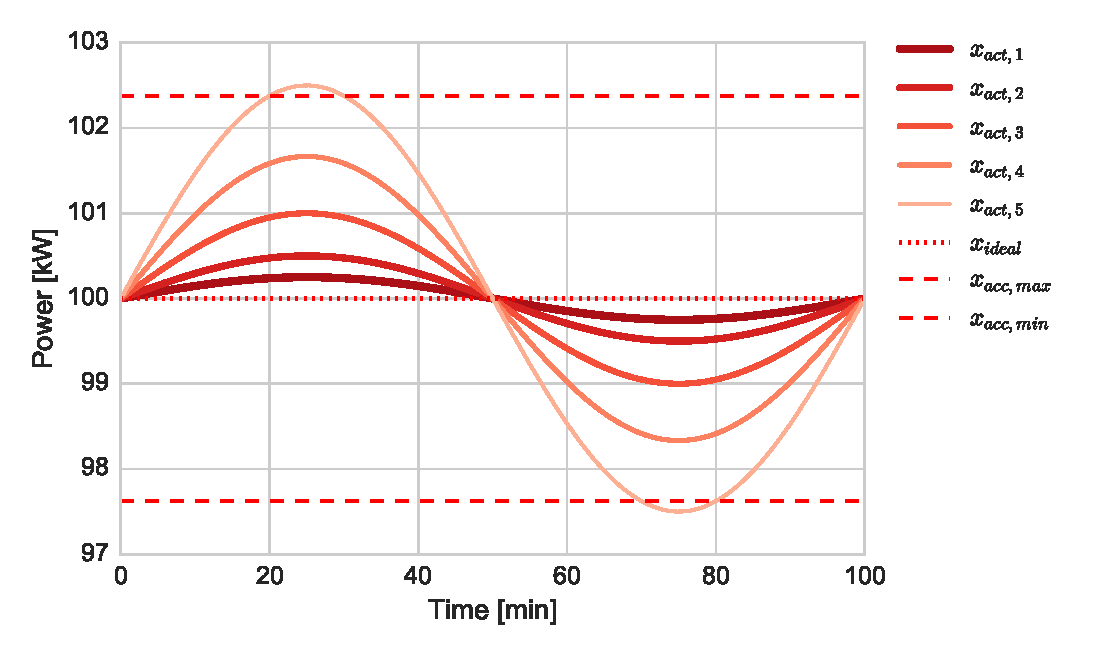
\includegraphics[width=1\columnwidth]{indextest_initial.eps}%
\label{subfig:indextest3}} \\
\subfloat[QoS for the services]{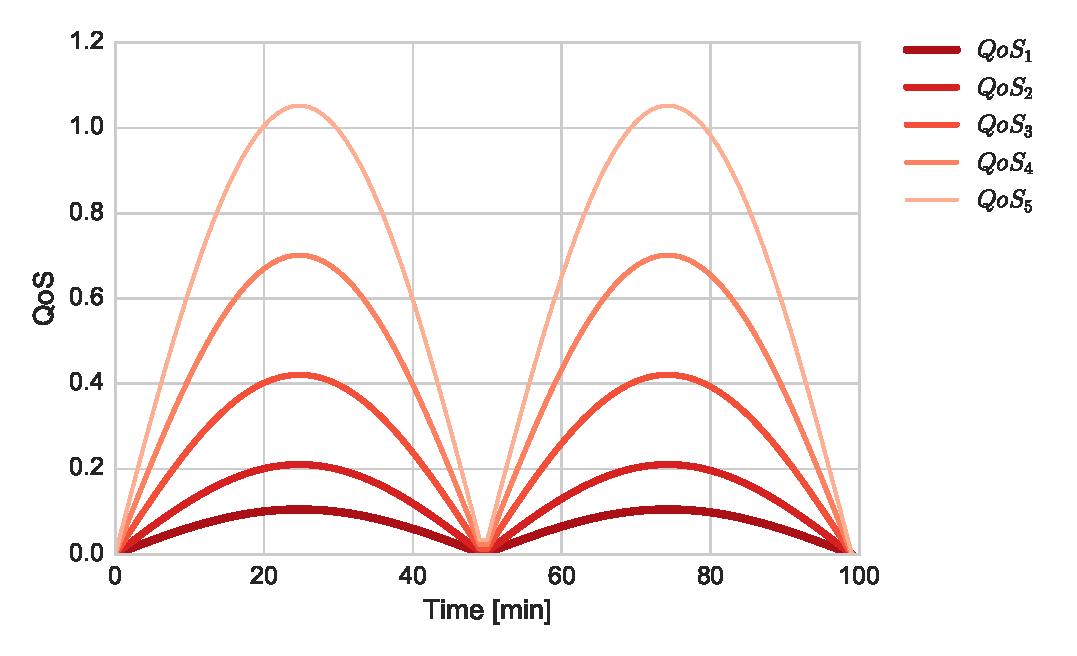
\includegraphics[width=1\columnwidth]{qostest_initial.eps}%
\label{subfig:qostest3}}
\caption[][1\baselineskip]{Test of the QoS definition where five aggregators deliver the same service for the same time horizons and with different performance.}
\label{fig:indextest3}
\end{figure}

\begin{margintable}%[-5\baselineskip]%[h!]
	\centering
	\begin{tabular}{cc}
		\toprule
		Aggregator & $\eta$ \\
		\midrule
		1 & 0.0740 \\
		2 & 0.1481 \\
		3 & 0.2962 \\
		4 & 0.4937 \\
		5 & 0.7308 \\
		\bottomrule
	\end{tabular}
	\caption{The values of $\eta$ for same service delivery horizons and different service performance.}
	\label{tab:qostest3}
\end{margintable}
%\FloatBarrier
The definition of $\eta$ takes the time horizon of service provision into account. This is done, so that the performance assessment gives a result that is scaled to the time scale of service delivery. For example, if two aggregators perform with an error of equal magnitude, but one aggregator is contracted to deliver the service on a shorter time horizon, the assessment of this aggregator should be worse than the one which was contracted for a longer period. This is shown in Figure~\ref{fig:indextest4} and Table~\ref{tab:qostest4}, where Aggregator 1 delivers the same service and the same error as Aggregator 2 but over half the delivery period.

\begin{figure}[htb!]
\centering
\subfloat[Simulated service delivery]{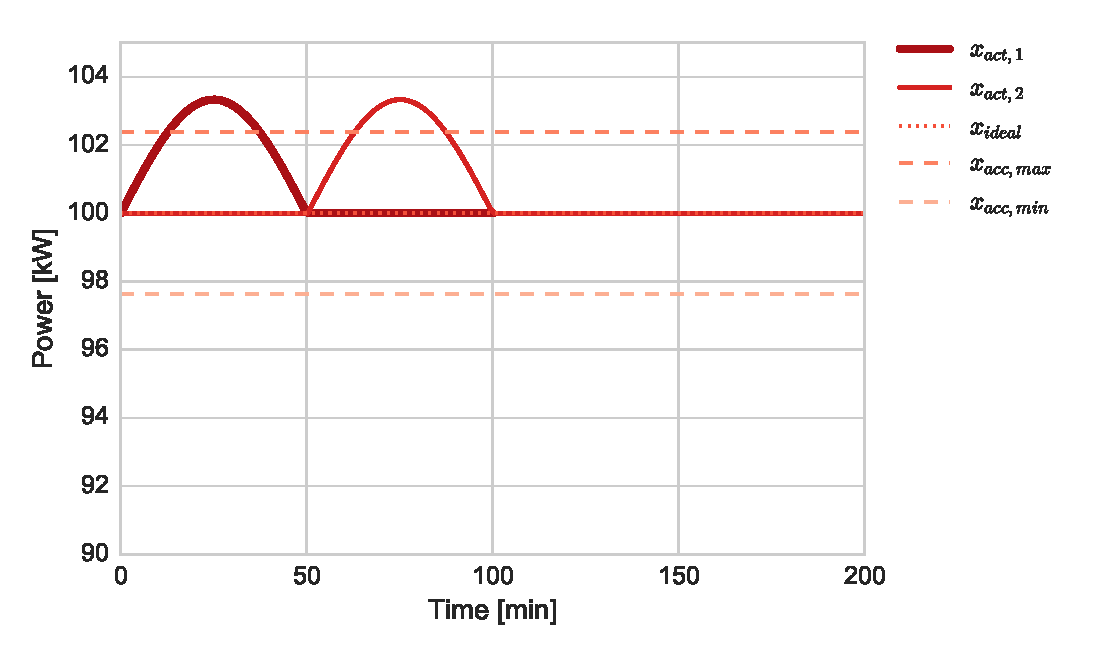
\includegraphics[width=1\columnwidth]{timenormtest.eps}%
\label{subfig:indextest4}}\\
\subfloat[QoS for the services]{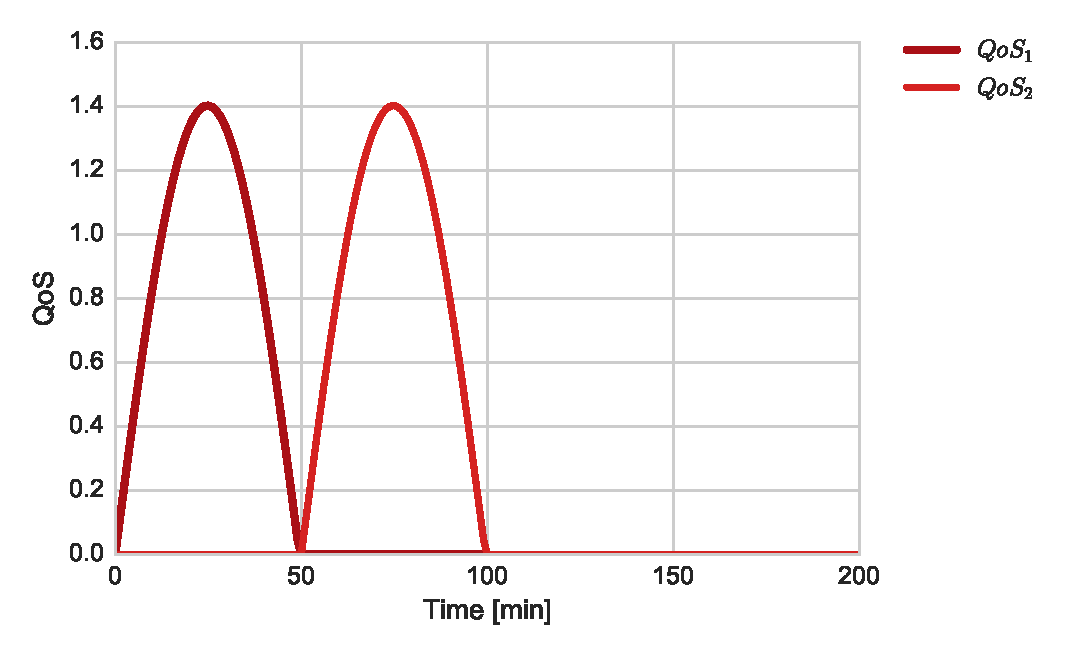
\includegraphics[width=1\columnwidth]{qostimenormtest.eps}%
\label{subfig:qostest4}}
\caption{Test of the QoS definition where 2 aggregators deliver the same service for different time horizons and with the same magnitude of error.}
\label{fig:indextest4}
\end{figure}

\begin{margintable}%[-1\baselineskip]%[h!]
	\centering
	\begin{tabular}{cc}
		\toprule
		Aggregator & $\eta$ \\
		\midrule
		1 & 0.3491 \\
		2 & 0.2469 \\
		\bottomrule
	\end{tabular}
	\caption{The values of $\eta$ for different service delivery horizons and with the same magnitude of error. Since $\eta$ is normalized with time, the shorter service is evaluated worse than the service delivered over the long time horizon.}
	\label{tab:qostest4}
\end{margintable}
%\FloatBarrier
Conversely, if two aggregators deliver a service on different time horizons and both have an error in service delivery which is \emph{proportionately} the same, the performance assessment will evaluate them to have equal performance. This is illustrated in Figure~\ref{fig:indextest1}, where five aggregators deliver a reference tracking service over different time horizons. All aggregators have the same proportionate error\footnote{This is ensured by using a sine as the ``actual'' performance of the aggregators, and each case is an extra period of the sine wave.} which leads to the same $\eta$, as can be seen in Table~\ref{tab:qostest1}. There is a slight increase in the values of $\eta$ due to numerical round off, which means that the precision of $\eta$ depends on the precision of the measurements. The amount of significant digits should be determined by the system operator or whichever entity is in charge of the service performance assessment.
\begin{figure}[htb!]
\centering
\subfloat[Simulated service delivery]{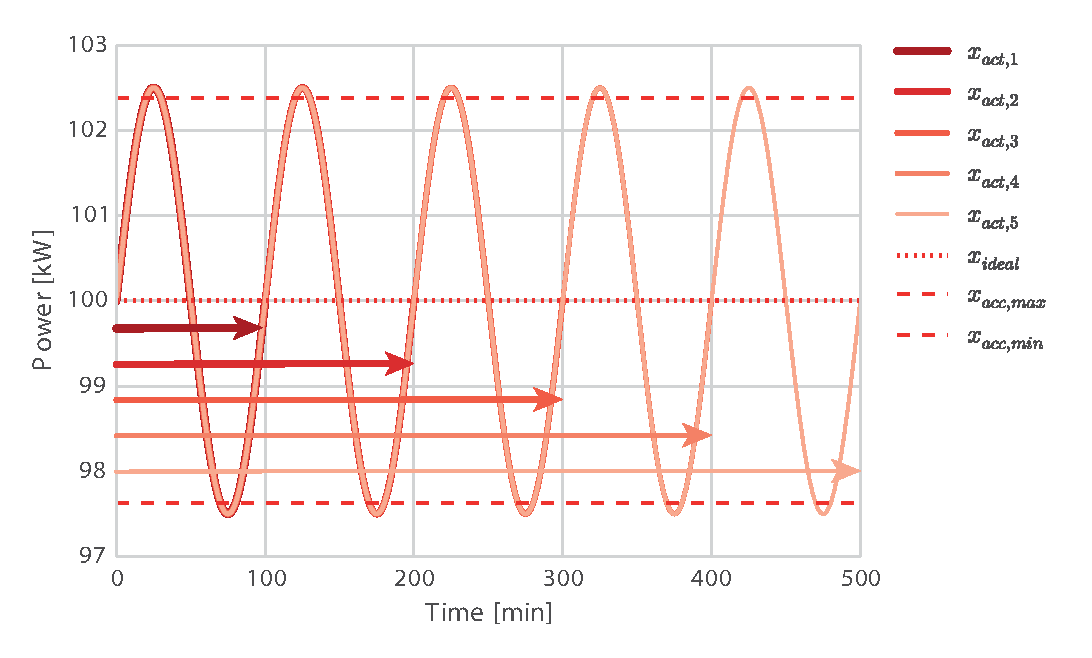
\includegraphics[width=1\columnwidth]{indextest_difftime_sameqos.eps}%
\label{subfig:indextest1}} \\
\subfloat[QoS for the services]{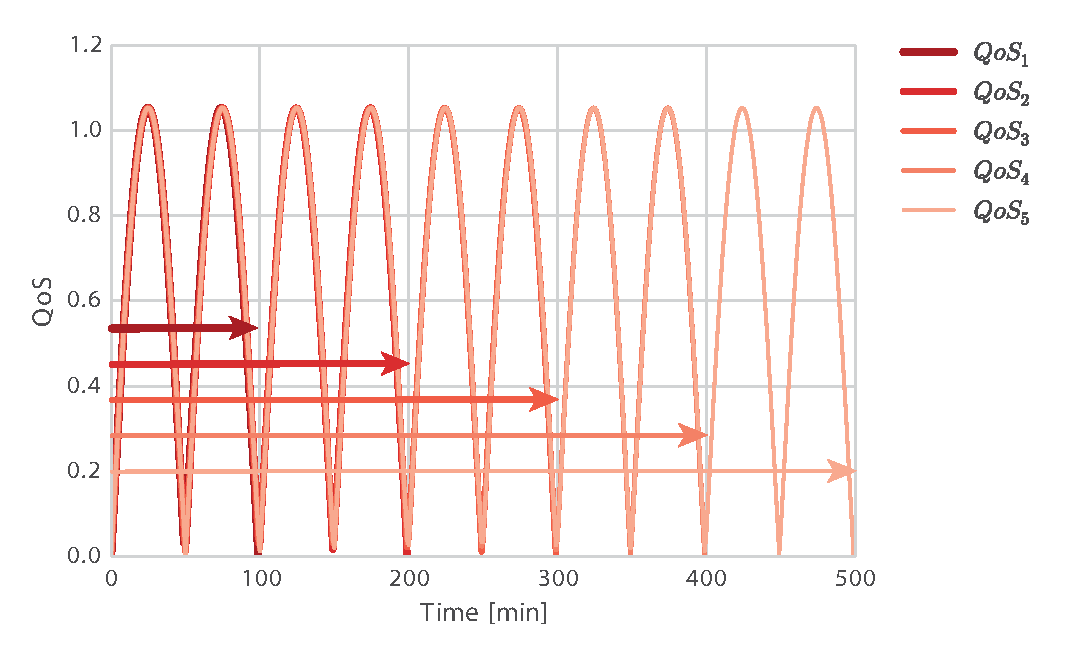
\includegraphics[width=1\columnwidth]{qostest_difftime_sameqos.eps}%
\label{subfig:qostest1}}
\caption{Test of the QoS definition where five aggregators deliver the same service for different time horizons and with the same performance.}
\label{fig:indextest1}
\end{figure}

\begin{margintable}%[15\baselineskip]%[h!]
	\centering
	\begin{tabular}{cc}
		\toprule
		Aggregator & $\eta$ \\
		\midrule
		1 & 0.7309 \\
		2 & 0.7327  \\
		3 & 0.7327  \\
		4 & 0.7333  \\
		5 & 0.7338 \\
		\bottomrule
	\end{tabular}
	\caption{The values of $\eta$ for different service delivery horizons. A numerical difference appears in the third decimal due to rounding error. The precision of $\eta$ depends on the measurement equipment of the flexibility asset.}
	\label{tab:qostest1}
\end{margintable}
%\FloatBarrier
Finally, Figure~\ref{fig:indextest2} and Table~\ref{tab:qostest2} show five aggregator delivering the same service for different time horizons and with different performance. It can be seen that truncating the \emph{QoS} when calculating $\eta$ means that $\eta$ alone can not be used for assessing if a service was delivered. Thus, the service verification index, described in the next section, must be taken into account in order to give a complete idea of service performance and delivery.
\begin{figure}[t!]
\centering
\subfloat[Simulated service delivery]{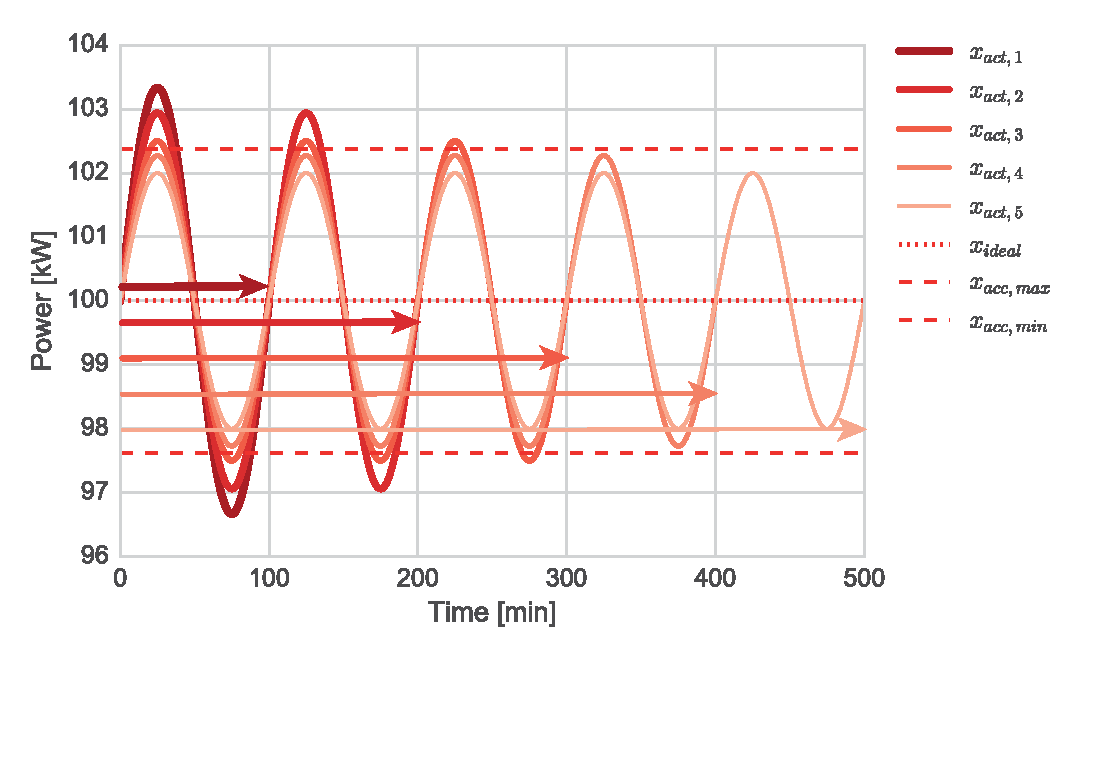
\includegraphics[width=1\columnwidth]{indextest_difftime_diffqos.eps}%
\label{subfig:indextest2}} \\
\subfloat[QoS for the services]{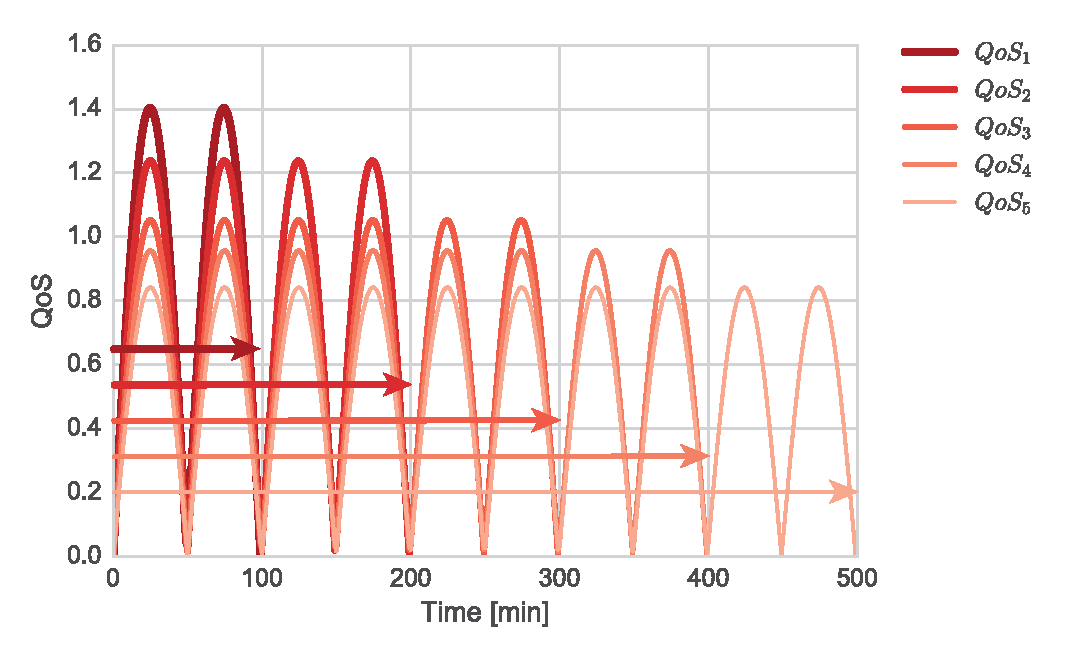
\includegraphics[width=1\columnwidth]{qostest_difftime_diffqos.eps}%
\label{subfig:qostest2}}
\caption{Test of the QoS definition where five aggregators deliver the same service over different time horizons and with different performance.
}
\label{fig:indextest2}
\end{figure}
\begin{margintable}%[-8\baselineskip]%[h!]
	\centering
	\begin{tabular}{cc}
		\toprule
		Aggregator & $\eta$ \\
		\midrule
		1 & 0.8199 \\
		2 & 0.7904  \\
		3 & 0.7333  \\
		4 & 0.6758  \\
		5 & 0.5949 \\
		\bottomrule
	\end{tabular}
	\caption{The values of $\eta$ over different service delivery horizons and different service performance.}
	\label{tab:qostest2}
\end{margintable}

%\FloatBarrier

\subsection{Service Verification Index}
Similar to the service performance assessment index, an index is defined for service verification\footnote{This index can also be interpreted as an index measuring non-delivery.} based upon \emph{QoS} whenever $QoS > 1$. A new non-delivery measure is introduced:
\begin{equation}
	ND(t) = QoS(t) - 1,\quad \forall QoS(t) > 1, \forall t.
\end{equation}
Using this new measure, the service verification index for \emph{K} amount of ancillary services, over a discrete time horizon of service delivery \emph{N}, is defined as:
\begin{equation}\label{eq:epsilonASmain}
	\epsilon^{AS} = \sum^{K}_{i=1} W^{AS}_i \sqrt{\frac{\sum^{N_i}_{t=0} \left( {ND^{AS}_{i,t}}^{2} \right)}{N_i}}
\end{equation}
where $\epsilon^{AS} \in [0,\infty]$ and $W^{AS}_i$ is the same as in Equation~\eqref{eq:was}. Similar to $\eta$, $\epsilon$ is also normalized to time.

The service verification for the index can also be defined for asset management services:
\begin{equation}\label{eq:epsilonAMSmain}
	\epsilon^{AMS} = \sum^{M}_{i=1} W^{AMS}_i \sqrt{\frac{\sum^{N_i}_{t=0} \left( {ND^{AMS}_{i,t}}^{2} \right)}{N_i}}
\end{equation}
where  \emph{M} is the size of the unit portfolio and $W^{AMS}_i$ corresponds to Equation~\eqref{eq:wams}. Following the definition of $\eta$, the verification index scales with time. This can be seen through the verification index values corresponding to Figure~\ref{fig:indextest1} in Table~\ref{tab:epstest1}. Again, due to numerical accuracy, only the second decimal number is significant.
\begin{margintable}%[h!]
	\centering
	\begin{tabular}{cc}
		\toprule
		Aggregator & $\epsilon$ \\
		\midrule
		1 & 0.0838 \\
		2 & 0.0839  \\
		3 & 0.0840  \\
		4 & 0.0840  \\
		5 & 0.0841 \\
		\bottomrule
	\end{tabular}
	\caption{The values of $\epsilon$ over different service delivery horizons with same delivery error, as shown in Figure~\ref{fig:indextest1}.}
	\label{tab:epstest1}
\end{margintable}

The two proposed indices have almost the same definition, the difference being that \emph{ND} is not truncated when estimating $\epsilon$. Table~\ref{tab:epstest2} shows the $\epsilon$ values corresponding to the example in Figure~\ref{fig:indextest2}, and shows clearly the definition of \emph{ND}, \ie values $QoS \leq 1$ are ignored, while $QoS > 1$ count as part of the non-delivery. Contrary to the service performance assessment index, the verification index does not have a clear limit for what is considered a verified serviced. For some services, \eg ancillary services, it is critically important that $QoS(t) \ll 1$, which would mean a requirement of $\epsilon \approx 0$. In other cases, $\epsilon > 0$ is tolerable to certain extent. The tolerance limit for $\epsilon$ should be defined in the contract agreements between aggregator and the entity acquiring the services.

\begin{margintable}[-5\baselineskip]%[h!]
	\centering
	\begin{tabular}{cc}
		\toprule
		Aggregator & $\epsilon$ \\
		\midrule
		1 & 0.3612 \\
		2 & 0.2512  \\
		3 & 0.0840  \\
		4 & 0.0  \\
		5 & 0.0 \\
		\bottomrule
	\end{tabular}
	\caption{The values of $\epsilon$ corresponding to Figure~\ref{fig:indextest2}.}
	\label{tab:epstest2}
\end{margintable}

%\begin{table}[h!]
%	\centering
%	\begin{tabular}{cc}
%		\toprule
%		Aggregator & $\epsilon$ \\
%		\midrule
%		1 & 0.3612 \\
%		2 & 0.2506  \\
%		3 & 0.0838  \\
%		4 & 0.0  \\
%		5 & 0.0 \\
%		\bottomrule
%	\end{tabular}
%	\caption{The corresponding values of $\epsilon$ to Figure~\ref{fig:indextest3}.}
%	\label{tab:epstest3}
%\end{table}

\section{Application to Service Verification}
\newsection{T}{he two indices defined} in the previous section have different applications. As stated in the introduction to the chapter, verification occurs at the prequalification phase, at the operation phase and at the settlement phase. The work during this project has focused on the use of the indices for prequalification and settlement. 

\subsection{Prequalification Verification}
In the case of prequalification, the indices form part of the assessment module of the validation framework presented in Figure~\ref{fig:MAINframework}. As such, the indices can evaluate the simulated results and return the $\eta$ and $\epsilon$ results. Since the simulations will be repeated enough times to gain a statistical certainty of the aggregator behavior, the verification of the simulated services will be a statistical value, \eg with a mean and a distribution.

\subsection{Settlement Verification}
Verification of delivered services occurs as a post-delivery analysis. For an aggregator, the verification of a delivered service will be done by the entity who bought the service, or a third party metering company. It is still an open question how the specific DER consumption/production will be measured, since in most cases the resource will be behind a common metering point, \eg the smart meter of a household. Also, current measurement requirements would force all resources to have expensive measurement equipment, of which the cost would far outweigh the profit of participating in the ancillary service markets. As part of an iPower demonstration event held at DTU Risø Campus in November 2014, a verification module was implemented, using the index definition of \cite{bondy2014performance}, for the verification of a DSO service. In this case, the consumption of the participating DER came only from flexible heating, and the measured consumption could be used to verify the service. An integration of the verification script to the code running the demonstration also showed that the same code could be used as a simple online performance monitoring tool.

\section{Conclusions on Performance Assessment}
The topic of performance assessment is important for the prequalification of aggregators, the monitoring of aggregator service delivery and the settlement of services. The presented indices are a tool that is useful for performance assessment. Although the concept of performance indices are not new in the power system, the established indices evaluate the overall system performance and reliability. While these indices provide a useful tool for system operators to evaluate their performance in maintaining a secure grid, they are not suited for the evaluation of aggregators. Therefore, the definition of these indices present a novel approach to the problem of evaluating the performance of aggregators.

A weakness in the presented work is that for verification of services, both indices must be used. The value of $\eta$ will always fall within the acceptable range $\eta \in [0,1]$ and it will be the value of $\epsilon$ which determines if the service is delivered. Still, $\eta$ gives an intuitive idea of how well the aggregator is performing within the limits stipulated within its service contract. $\epsilon$ does not have this same intuitive meaning, but in that sense it is not different from other fit measures used in statistics.

Future work will focus on a re-implementation of the verification module for the laboratory, incorporating the indices defined in \cite{bondy2016method}. Also, research must be done with respect to how to measure the individual DER consumption in an economically feasible way, with enough resolution to do settlement verification.
% chapter Service Verification (end)

